%!TEX root = main.tex
\section{Einführung}
		
	\begin{minipage}[t][\textheight][t]{0.76\textwidth}

	Diese Arbeit beschäftigt sich mit der Verallgemeinerung von Knoteninvarianten. Das Ziel ist die Ausarbeitung des Beweises von McMullens Abschätzung (2002) aus \cite{MCMULLEN.2002} der Alexander-Norm und der Thurston-Norm auf 3-Mannigfaltigkeiten. Der Kontext der Theorie der 3-Mannigfaltigkeiten beinhaltet insbesondere große Teile der Knoten- und Verschlingungstheorie, in der 3-Mannigfaltigkeiten aus Komplementen von Knoten oder Verschlingungen in der 3-Sphäre hervorgehen. In diesem Sinne sollen das Alexander Polynom und das Knotengeschlecht verallgemeinert werden.

	Die Theorie der Knoten beschäftigt sich mit Äquivalenzklassen von Knoten und dem Finden von Invarianten solcher Äquivalenzklassen. In der differenzierbaren Kategorie bezeichnet man mit einem Knoten eine glatte orientierte Einbettung $S^1\into S^3$ und man bezeichnet zwei Knoten als äquivalent, wenn ein orientierungserhaltener Diffeomorphismus $S^3\to S^3$ existiert, der beide Knoten ineinander überführt. Als häufig betrachtete Invariante hat sich die orientierte Diffeomorphieklasse der kompakten 3-Mannigfaltigkeit ergeben, die man das Knotenkomplement nennt. Dieses entsteht durch Entnehmen einer offenen Tubenumgebung des eingebetteten Knotens $S^1 \into S^3$ und ist eine naheliegende Knoteninvariante, das bedeutet äquivalente Knoten haben diffeomorphe Knotenkomplemente durch einen orientierungserhaltenden Diffeomorphismus. Häufig stellen sich Knoteninvarianten lediglich als Invarianten der Knotenkomplemente heraus. Um die Qualität und Feinheit dieser Invarianten zu beurteilen, ist es zunächst wichtig die des Knotenkomplements zu beurteilen. Dies ist natürlich eine relevante Frage, schließlich gibt es unzählige Resultate . 1989 zeigen Gordon und Luecke~\cite{Gordon.1989}, dass Knoten sogar durch ihr Knotenkomplement in ihrer Klasse bestimmt sind, es sich bei dem Knotenkomplement also um eine vollständige Knoteninvariante handelt. Manche Invarianten enstanden also aus rein homologischen Eigenschaften von 3-Mannigfaltigkeiten, andere wiederum entstanden speziell für 3-Mannigfaltigkeiten, die einen Torus als Rand haben. Um letztere soll es auch in dieser Arbeit gehen.

	Alexander definiert 1928 eine topologische Invariante des Knotenkomplements \cite{Alexander.1928}, die einem Knotenkomplement eine Klasse von Laurentpolynomen mit eindeutigem Grad zuordnet. 1934 stellt Seifert in seiner Arbeit "`Geschlecht von Knoten"'~\cite{Seifert.1934} mit dem Geschlecht eine Invariante vor, die die minimale Komplexität einer orientierten eingebetteten Fläche berechnet die den Knoten aufspannt (nach der Klassifikation von Flächen wird diese in Abhängigkeit des Geschlechts gemessen) und eine Konstruktion für die Existenz solcher Flächen. Dieses Knotengeschlecht liefert die Möglichkeit jeden Knoten von dem Unknoten zu unterscheiden. Natürlich liefert die sogennante Seifert-Konstruktion eine Fläche mit Geschlecht, jedoch ist es ein deutlich komplizierteres Anliegen, wenn man zeigen möchte, dass eine gefundene Fläche in ihrer Komplexität nicht unterboten werden kann. Entsprechend günstig erweist sich Seifert's Resultat, dass der Grad des Alexander Polynoms eines Knoten eine untere Schranke für sein Geschlecht definiert. 


	\vfill
	\begin{minipage}[t]{0.7\textwidth}
		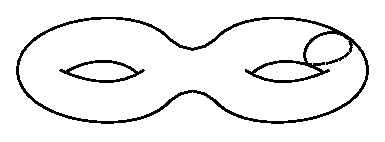
\includegraphics{zyklbott} 
	\end{minipage}
	\begin{minipage}[t]{0.2\textwidth}
	\vspace{-1cm}
	\huge$\longleftarrow$
	\vfill

	\end{minipage}
	\vspace{.63cm}
		\captionof{figure}{Unendlich zyklische Überlagerung} \label{fig:zykl}
	\end{minipage}
	\hfill
	\begin{minipage}[t]{0.2\textwidth}
	\vfill \begin{flushright}
		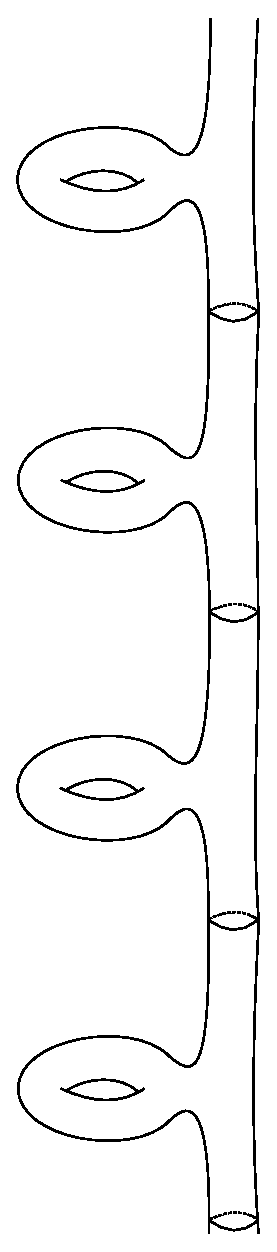
\includegraphics{zyklright} 
	\end{flushright}
	\end{minipage}
    
	Der wesentliche Gegenstand dieser Arbeit ist die Verallgemeinerung dieser auf Knotenkomplementen definierten Invarianten zu Invarianten auf kompakten orientierbaren 3-Mannigfaltigkeiten mit Rand, der maximal aus Tori besteht. Für diese Invarianten stellt McMullen~\cite{MCMULLEN.2002} fest, dass sich auch die oben erwähnte Abschätzung aus der Knotentheorie verallgemeinern lässt. Diese Arbeit beschäftigt sich mit genau diesem Resultat, welches dieser Arbeit als Haupttheorem~\ref{thm:haupttheorem} zugrunde liegt.

    Es stellt sich heraus, dass alle betrachteten Invarianten eine enge Beziehung zu unendlich zyklischen Überlagerungen haben. Diese können etwa durch Aufschneiden an einer 1-kodimensionalen Untermannigfaltigkeit gewonnen werden, siehe zum Beipsiel Abbildung~\ref{fig:zykl}. Diese Abbildung ist für die Intuition erheblich --- man könnte dem Leser fast raten, vor und nach jedem Kapitel die Abbildung~\ref{fig:zykl} zu betrachten und immer wieder neu zu reflektieren.

	Die ersten Kapitel beschäftigen sich mit der Definition, Konstruktion und der algebraischen Natur der Alexander-Norm und Thurston-Norm. Während die Alexander-Norm den Grad des Alexander Polynoms einer Seifert-Fläche (aufgefasst als Lefschetz duale Homologieklasse eines Erzeugers der ersten Kohomologie eines Knotenkomplementes) verallgemeinert auf eingebetteten orientierten Flächen auswertet, so soll die Thurston-Norm die minimale Komplexität einer eingebetteten orientierten Fläche bestimmen. Diese beiden Invarianten werden per Poincaré und Lefschetz Dualität als Halbnormen auf $H^1(M) \cong H_2(M,\partial M)$ betrachtet.

	Anschließend widmet sich dem Beweis des Haupttheorems ein eigenes Kapitel. Der Beweis ist an die Beweisführung aus~\cite{MCMULLEN.2002} angelehnt und beinhaltet eine Reihe Modifikationen und Ergänzungen. 

	Abschließend beschäftigt sich das letzte Kapitel mit der genaueren Betrachtung des Beweises, beinhaltet aber auch Anwendungen und konkrete Beispiele.

    Bei der Alexander-Norm eines Homomorphismus in $\Hom(\pi_1(M),\ZZ)$ handelt es sich um den Grad des zugehörigen Alexander Polynoms und die Thurston-Norm weist einem solchen Homomorphismus die minimale Komplexität einer Poincaré-Lefschetz dualen eingebetteten Fläche zu. Ohne die genauere Definition hier zu nennen (siehe hierzu Kapitel~\ref{sec:alexdefs}), soll nun das Theorem vorgestellt werden, dessen Beweis in dieser Arbeit behandelt wird.
    \begin{thm}[McMullen]
    \label{thm:haupttheorem}
    	Sei $M$ eine kompakte, zusammenhängende, orientierbare Mannigfaltigkeit der Dimension 3. Falls der Rand dieser Mannigfaltigkeit nicht leer ist, so soll er aus einer Kollektion von Tori bestehen. Dann gilt folgende Abschätzung für die Alexander-Norm und die Thurston-Norm $\alex \cdot ,\thur \cdot : H^1(M;\ZZ) \to \RR$ der 3-Mannigfaltigkeit:
    	\[
    		\alex \phi \leq 
    		\begin{cases}
    			\thur \phi + 1+ b_3(M) &\text{, falls } b_1(M)\leq 1 \text{ und } \phi: \pi_1(M) \onto \ZZ \\
    			\thur \phi &
    		\end{cases}
    	\]
    	Entsteht $\phi$ als Rückziehung einer Faserung $M\to S^1$, so gilt Gleichheit.
    \end{thm}